\subsection{User Interfaces}
Our application will be mainly developed as a Web Application, so the user can access to \emph{Travlendar+} services with a Web Browser. Furthermore, we want to develop an application for Android and IOS for a better user experience on mobile devices. What follows are some mock up pictures related to both the Web Application and the Mobile Application. The aim is to provide a clear visualization of what the main functionalities of the System are and how the user will interact with them.   
\newpage
\subsection*{Log in}
In the two images below there are the log in screens from the \emph{Travlendar+} Web and Mobile applications. In both cases, the visitor user may easily insert his Username and Password to log in into the System.  

\begin{figure}[H]
    \centering
    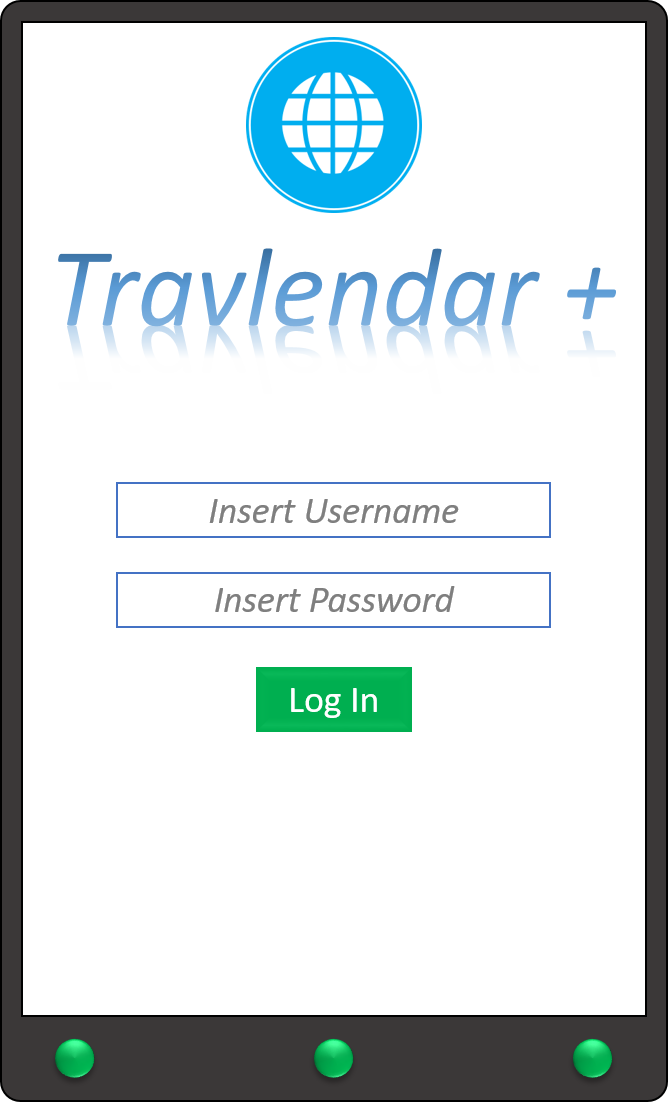
\includegraphics[scale=0.25]{Pictures/Mockups/AppLogin.png}
    \caption{Login from the mobile application}
\end{figure}

\begin{figure}[H]
    \centering
    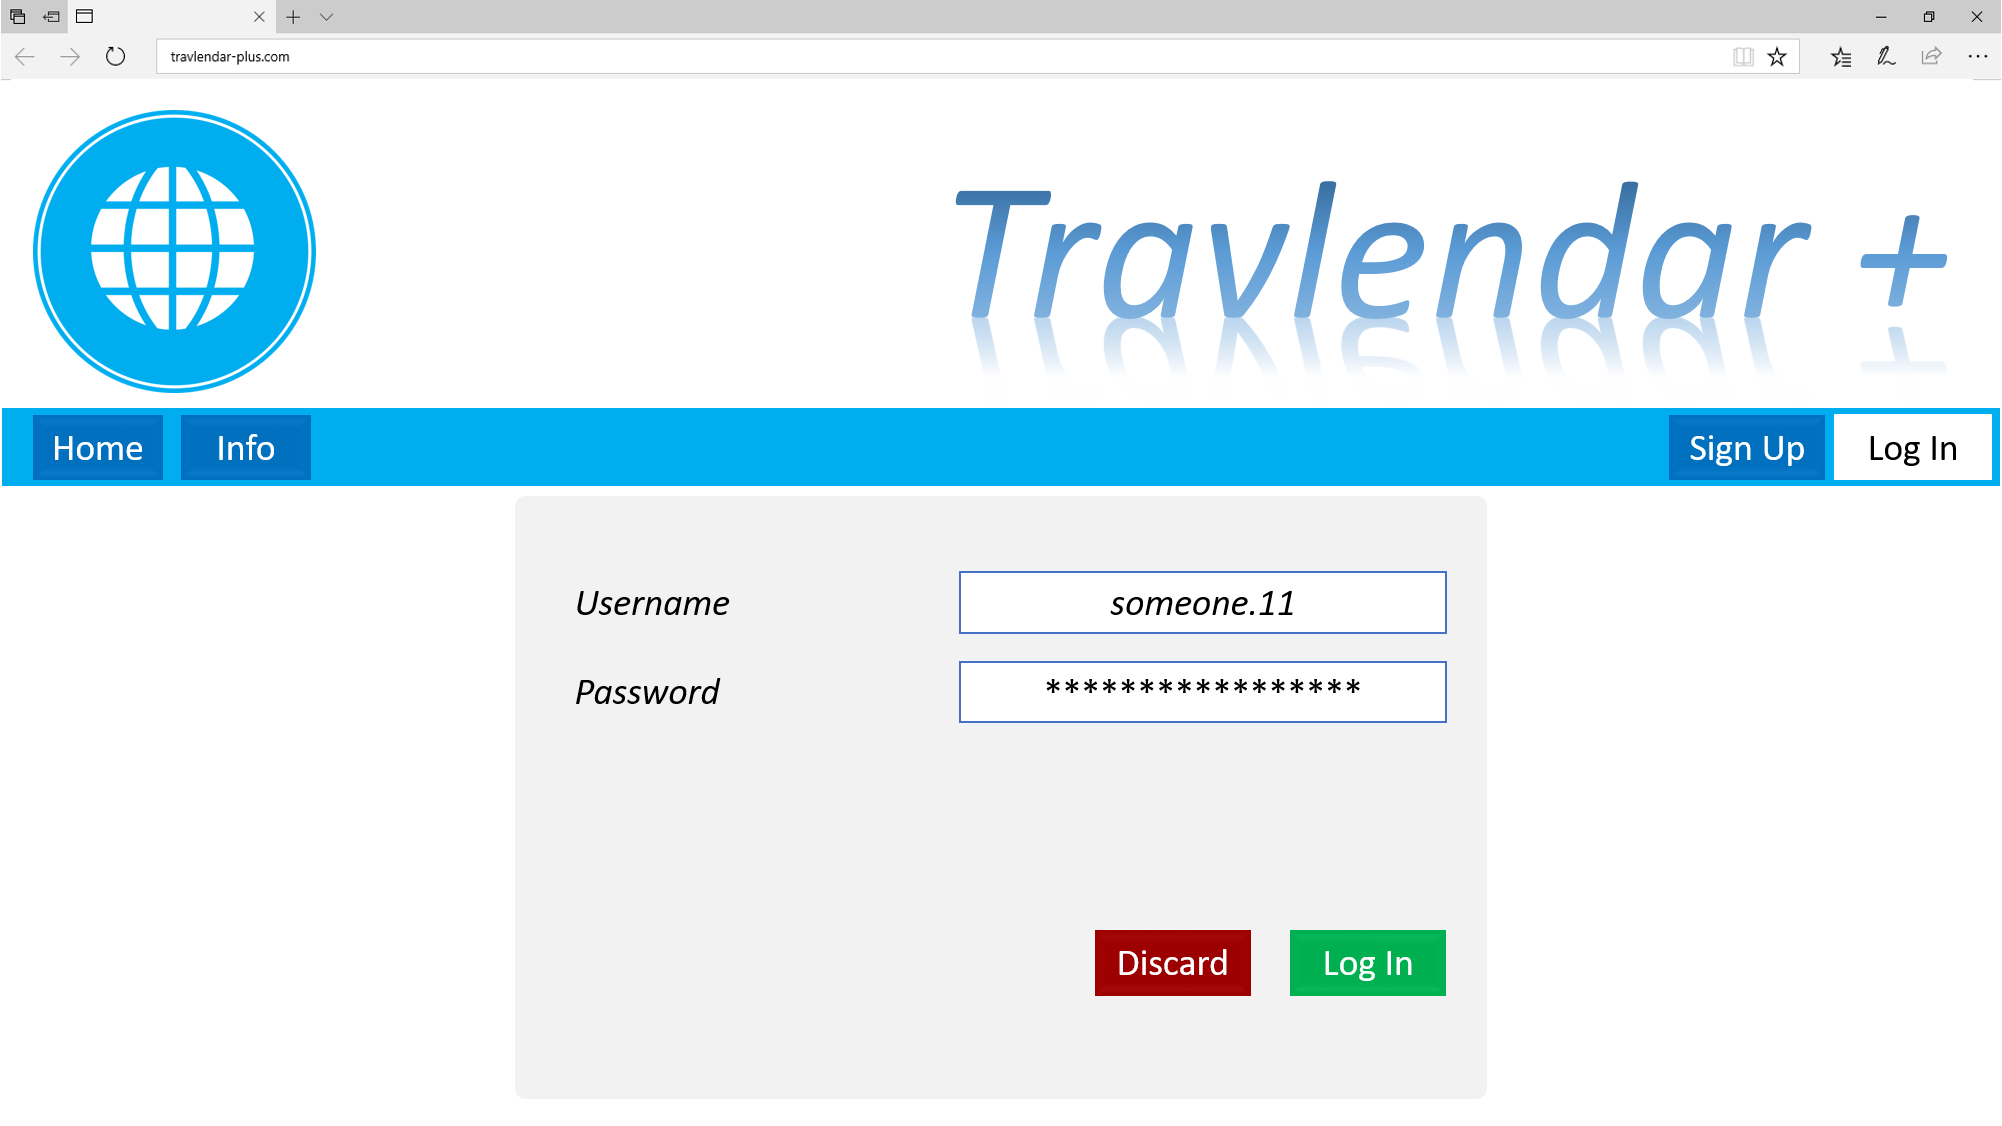
\includegraphics[scale=0.25]{Pictures/Mockups/SiteLogin.png}
    \caption{Login from the web page}
\end{figure}

\subsection{Calendar}
In the images below is represented a possible calendar rendering from both the \emph{Travlendar+} Web and Mobile applications. In these pages the user can have a look at the scheduled tasks, changing if he prefers the time granularity, from weekly to daily or monthly. In these screens the user will be able to select a task simply by clicking on it. In addition, on the Mobile application it will be possible to access a menu by swiping from the left to the right part of the screen.   

\begin{figure}[H]
    \centering
    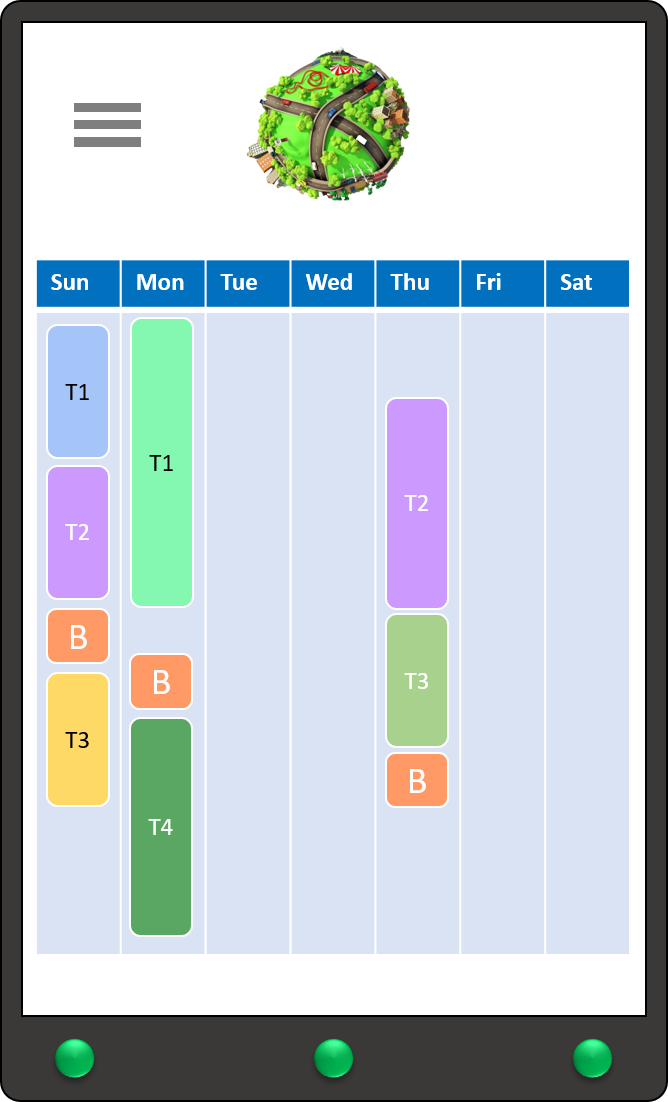
\includegraphics[scale=0.3]{Pictures/Mockups/AppCalendar.png}
    \caption{Calendar render on mobile device}
\end{figure}

\begin{figure}[H]
    \centering
    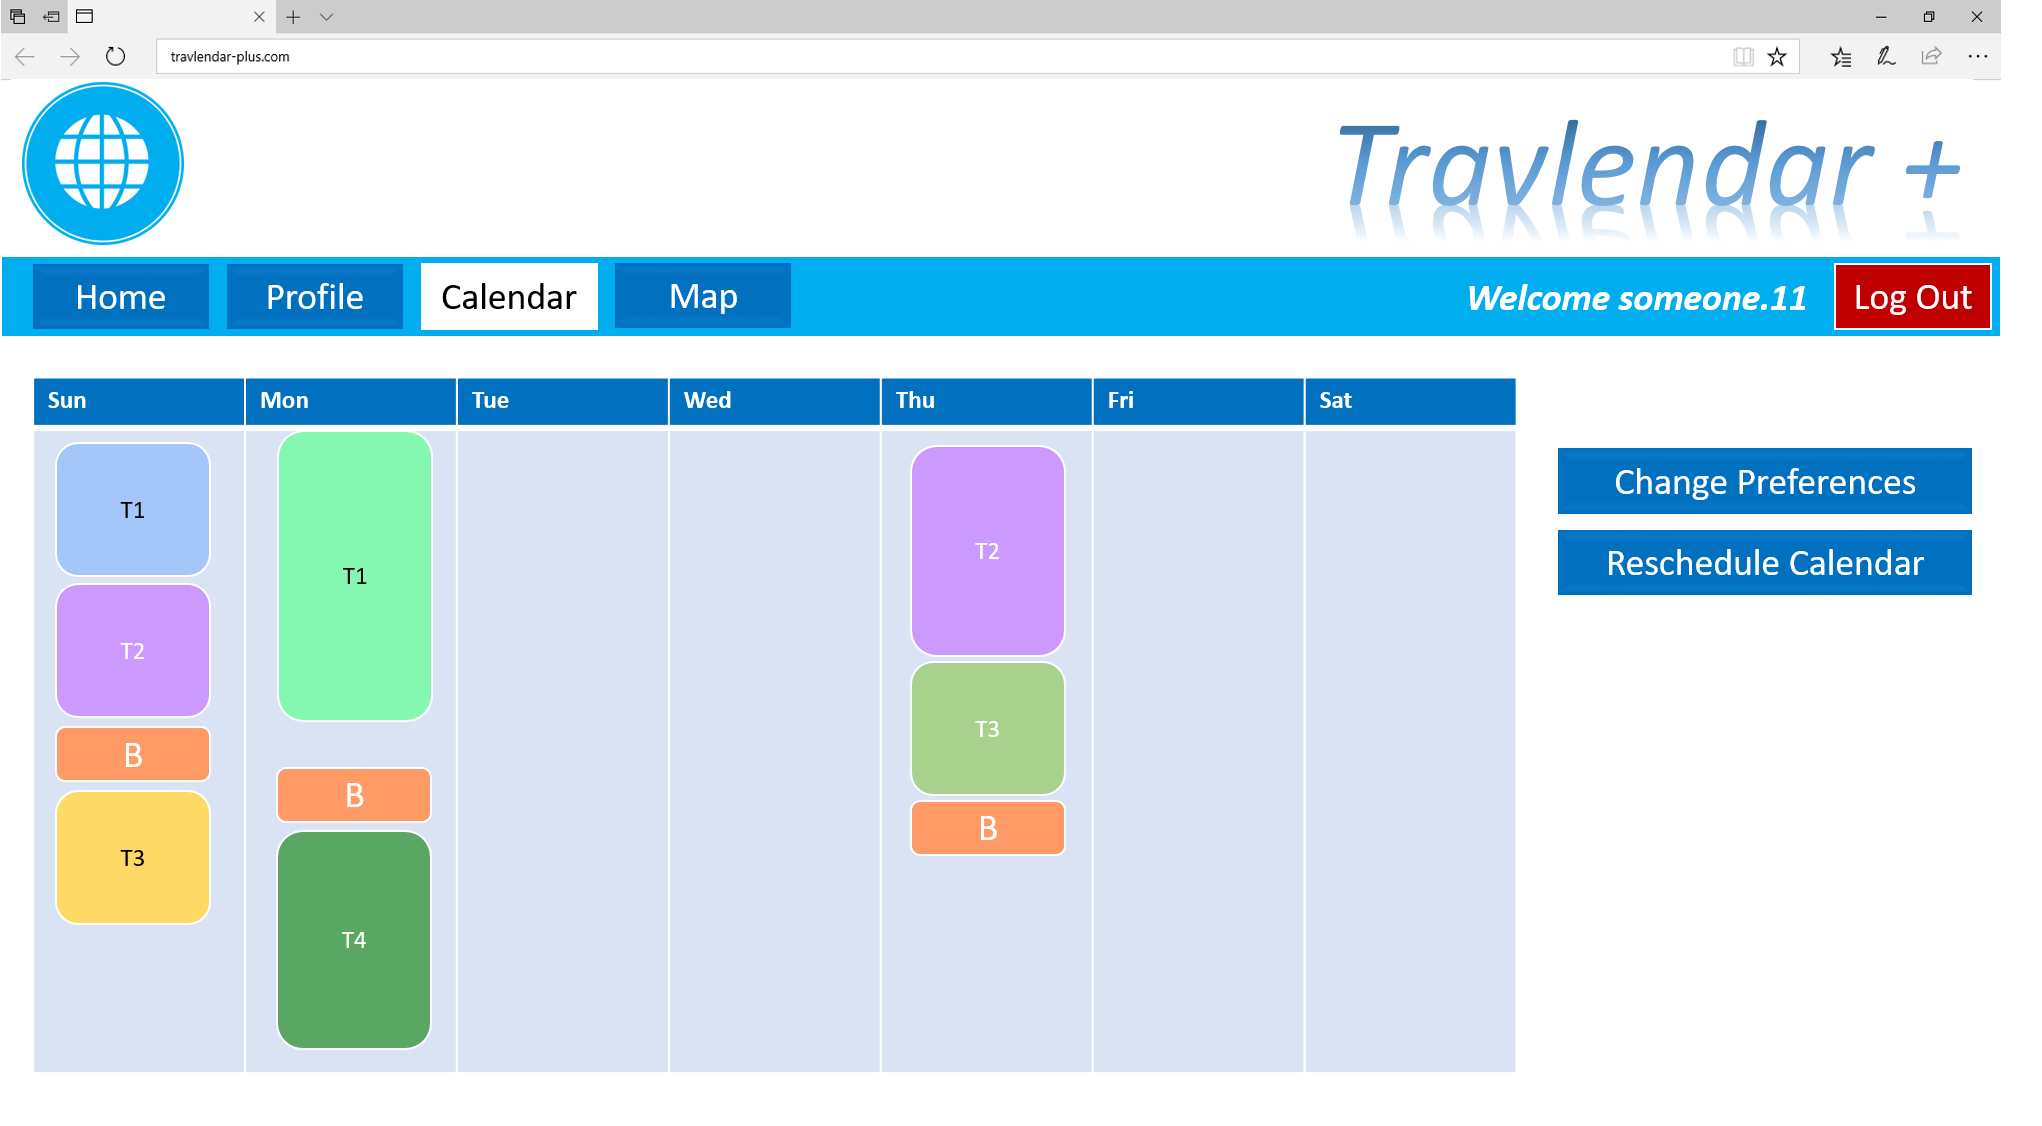
\includegraphics[scale=0.25]{Pictures/Mockups/SiteCalendar.png}
    \caption{Calendar render on web page}
\end{figure}

\begin{figure}[H]
    \centering
    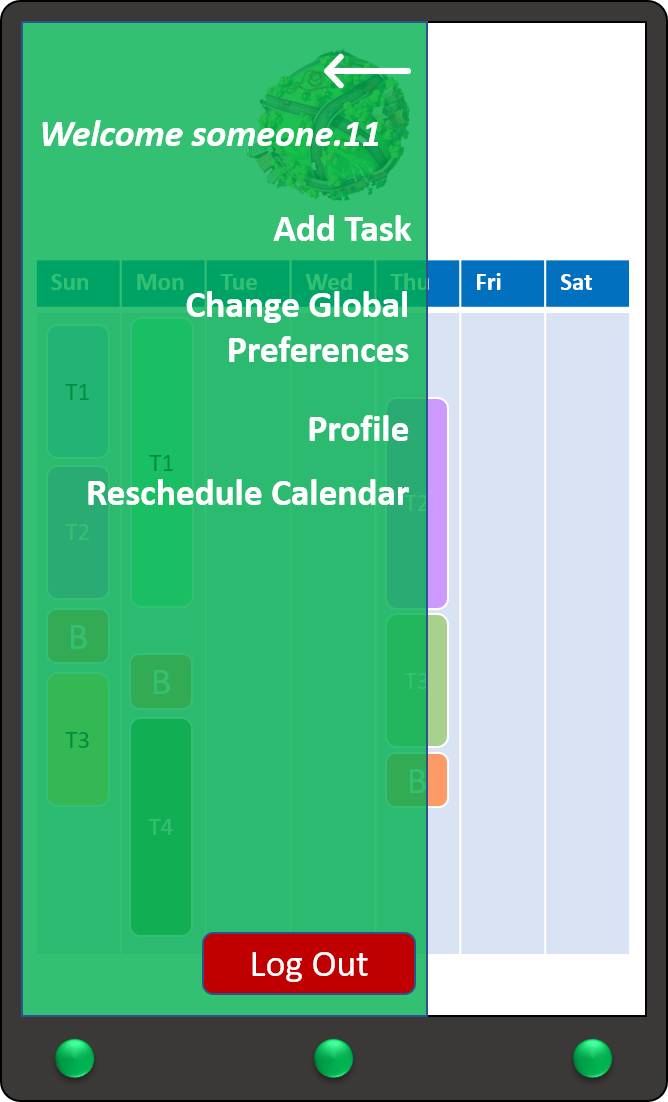
\includegraphics[scale=0.3]{Pictures/Mockups/AppMenu.png}
    \caption{Main menu on mobile device}
\end{figure}

\subsection{Task Modification}
From the images below it's possible to see a rendering for the task modification screen. In these pages the user will be able to change task's preferences, task's time and date. It will also be possible to access the Travel Map pages which are better explained in the following subsection.

\begin{figure}[H]
    \centering
    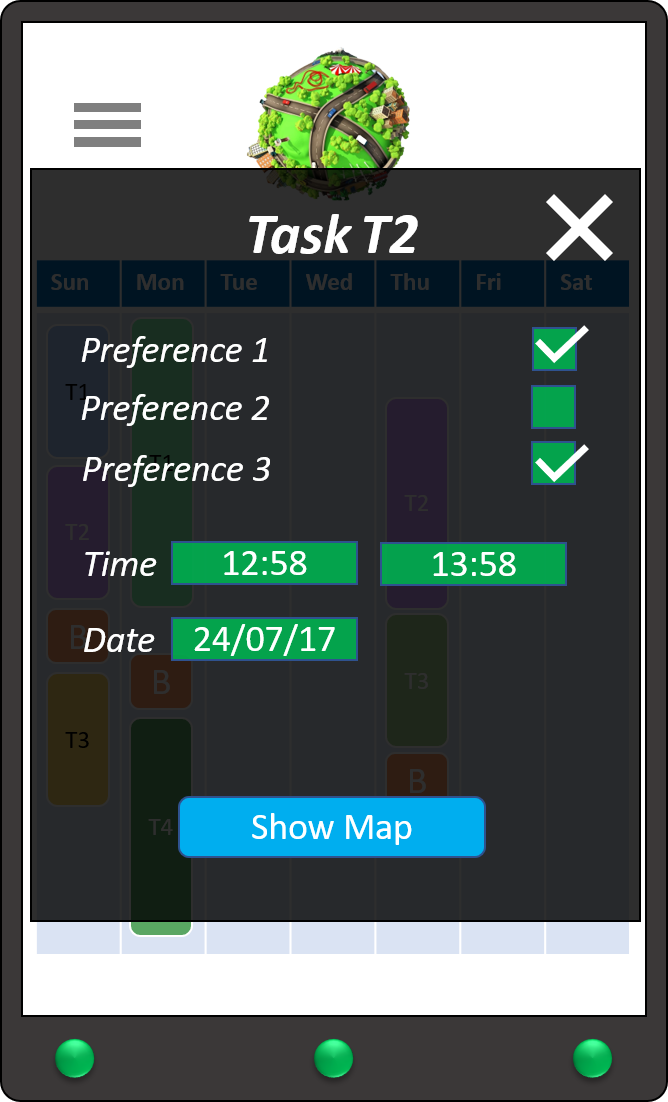
\includegraphics[scale=0.3]{Pictures/Mockups/AppTask.png}
    \caption{Task modification on mobile device}
\end{figure}

\begin{figure}[H]
    \centering
    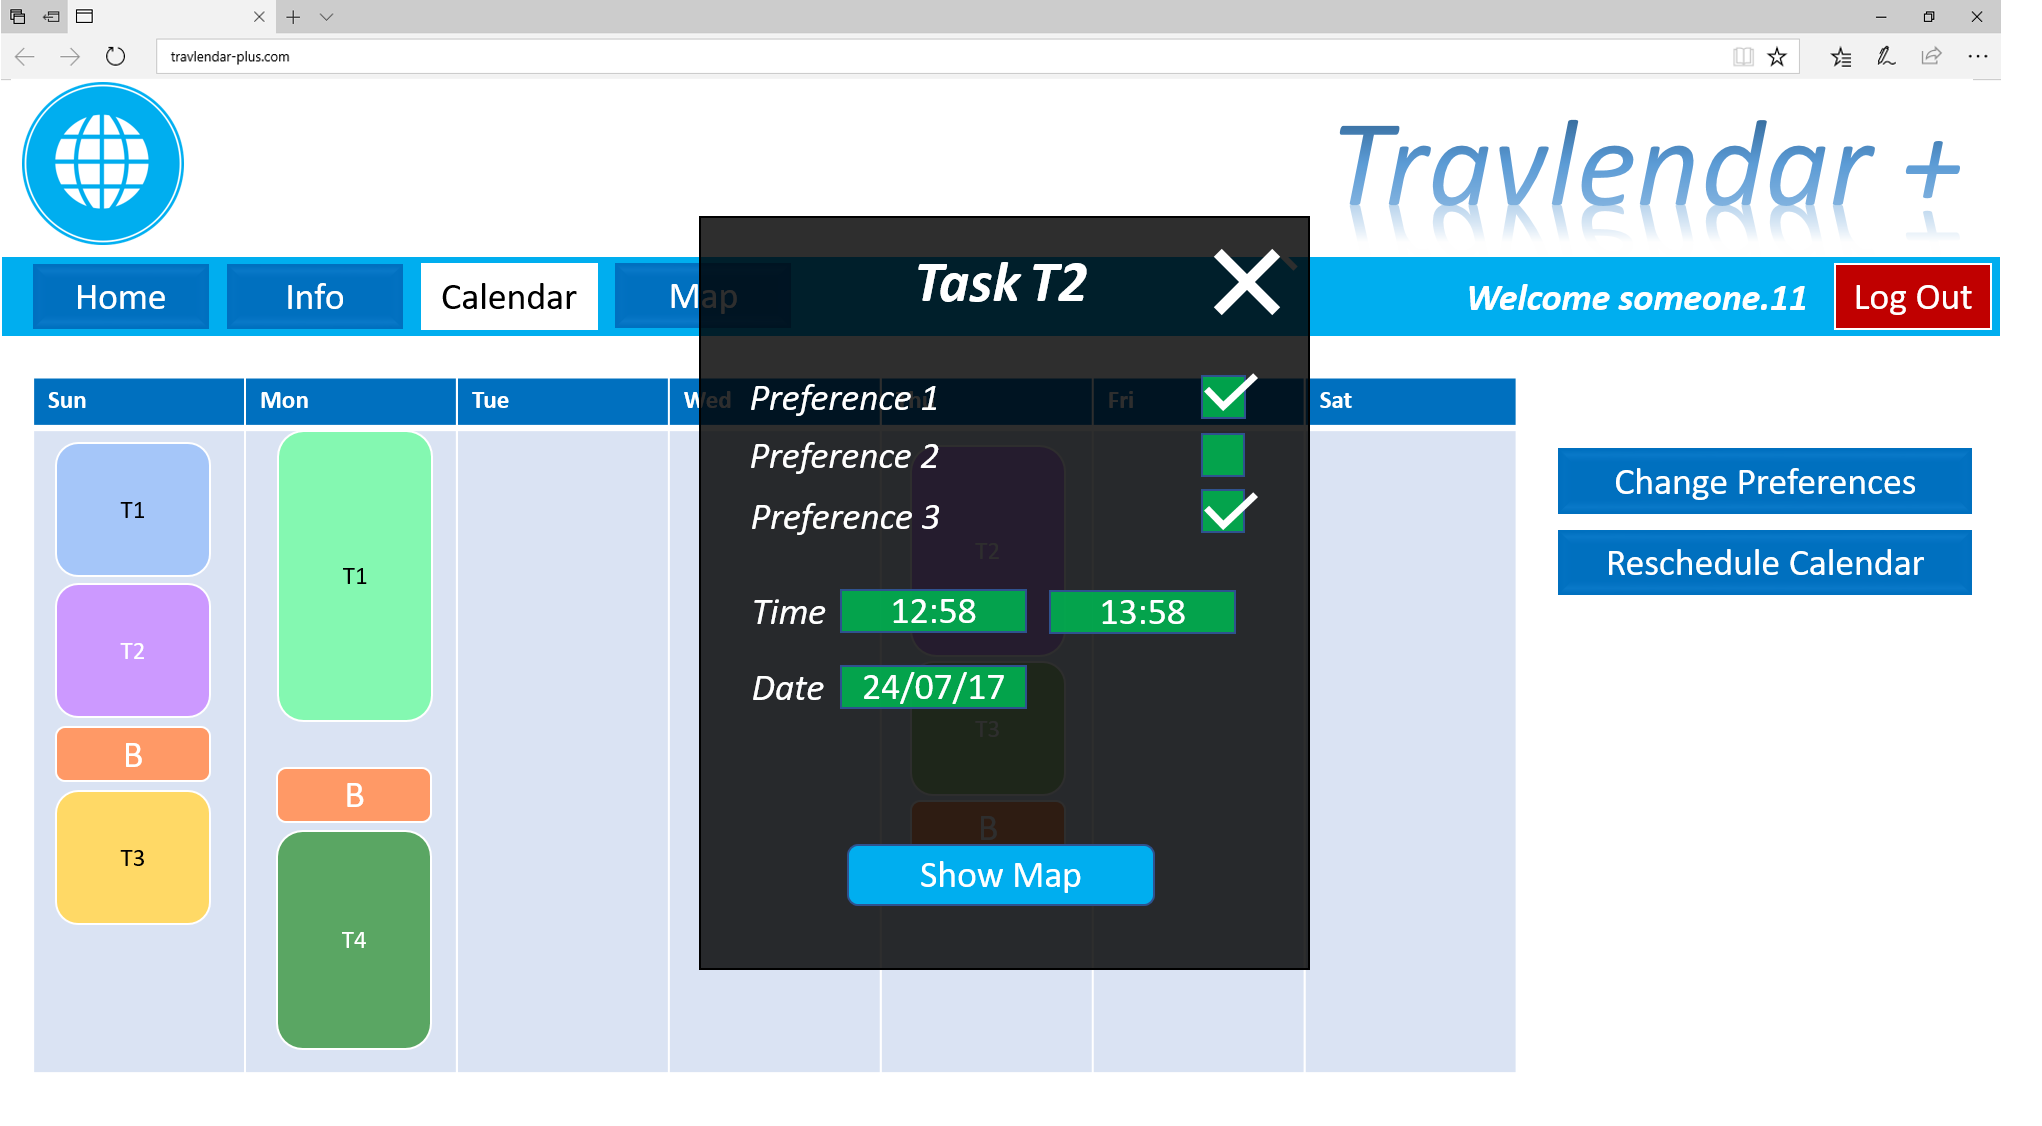
\includegraphics[scale=0.25]{Pictures/Mockups/SiteTask.png}
    \caption{Task modification on web page}
\end{figure}

\subsection{Task Travel Information}
In these last two pictures it's possible to see the screens related to the Travel information, from these pages the user can have a look at the travel solution scheduled for each task. From this page it's also possible to be redirected to an appropriate site or application for finalizing the purchase of a ticket or to rent a vehicle.   

\begin{figure}[H]
    \centering
    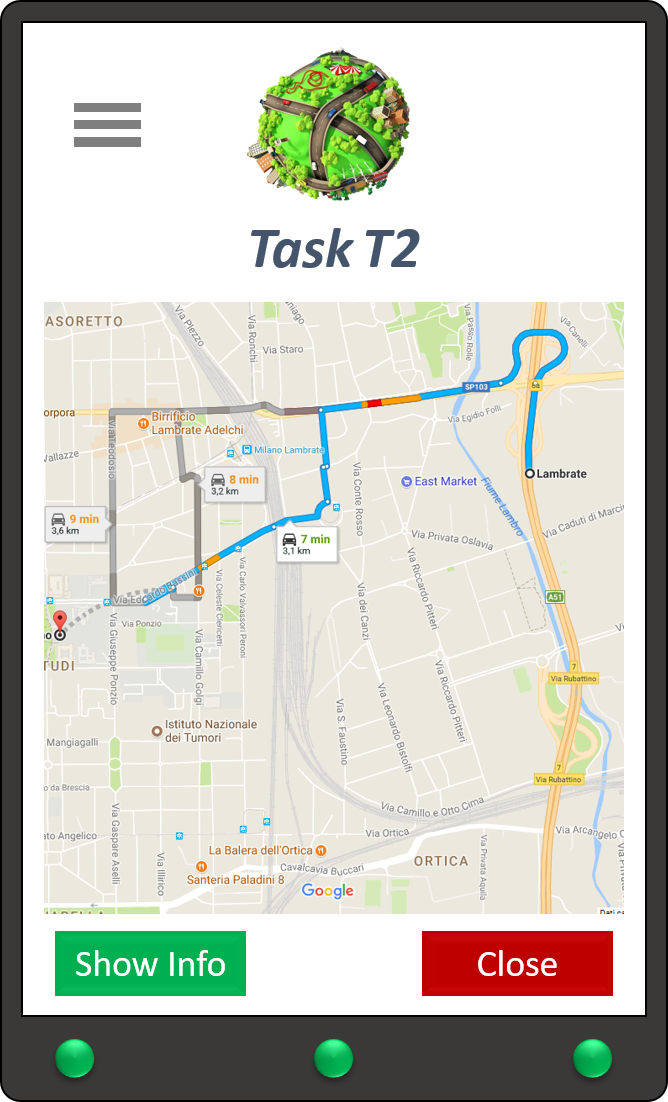
\includegraphics[scale=0.3]{Pictures/Mockups/AppMap.png}
    \caption{Map render and road information on mobile device}
\end{figure}

\begin{figure}[H]
    \centering
    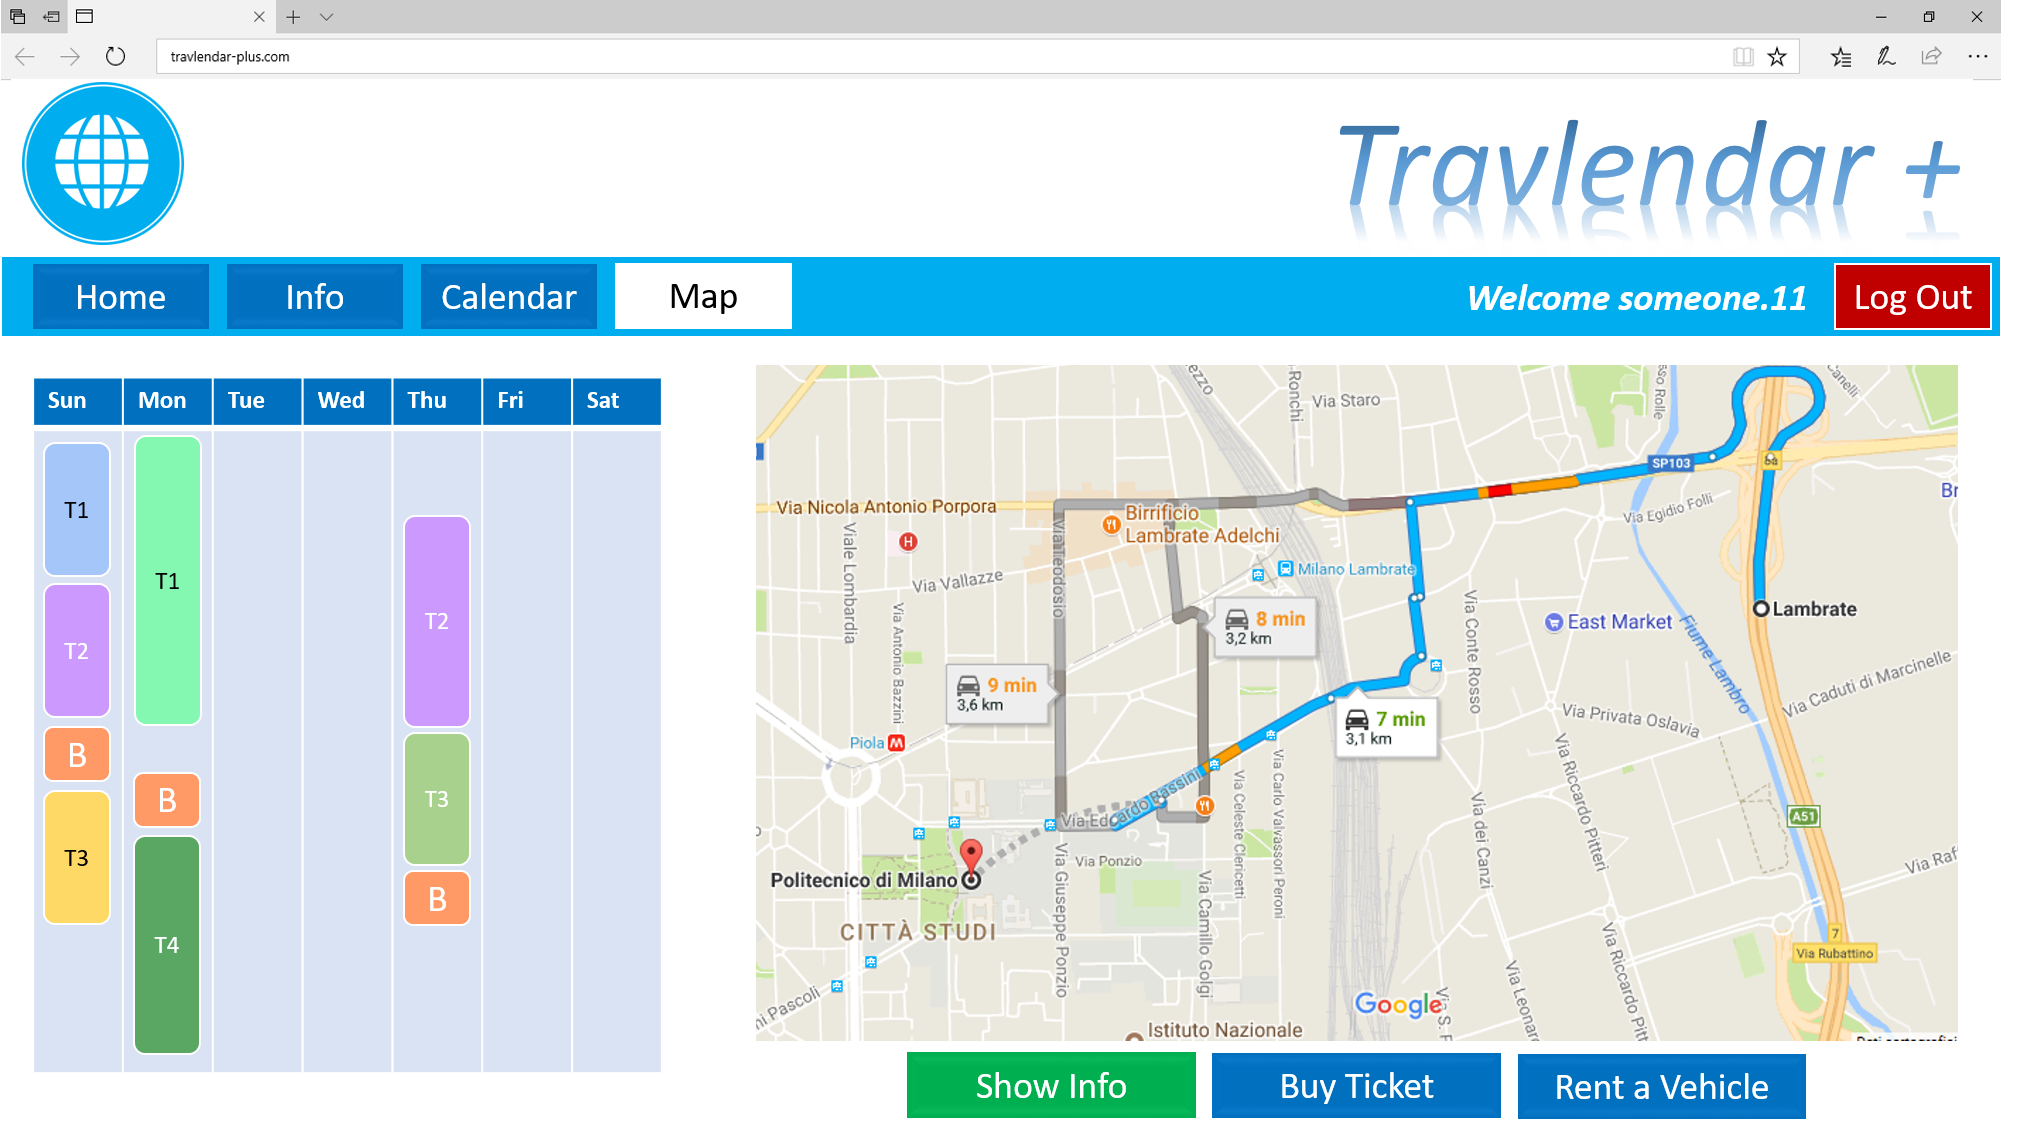
\includegraphics[scale=0.25]{Pictures/Mockups/SiteMap.png}
    \caption{Map render and road information on web page}
\end{figure}